\begin{frame}{Kinematic Fit}
\begin{columns}
\column{0.5\textwidth}    

\begin{itemize}
    \item Consist of calibration of the HH system
balance in the transverse plan.
    \item Profit from $m_{\gamma\gamma}$ resolution to
improve $m_{bb}$ resolution.

    \item Constrain the $P_{x,y}^{HH+jets}$, using a
likelihood, since additional jets are
an important part of HH system.
\end{itemize}

    
\column{0.5\textwidth}    
\begin{figure}
    \centering
    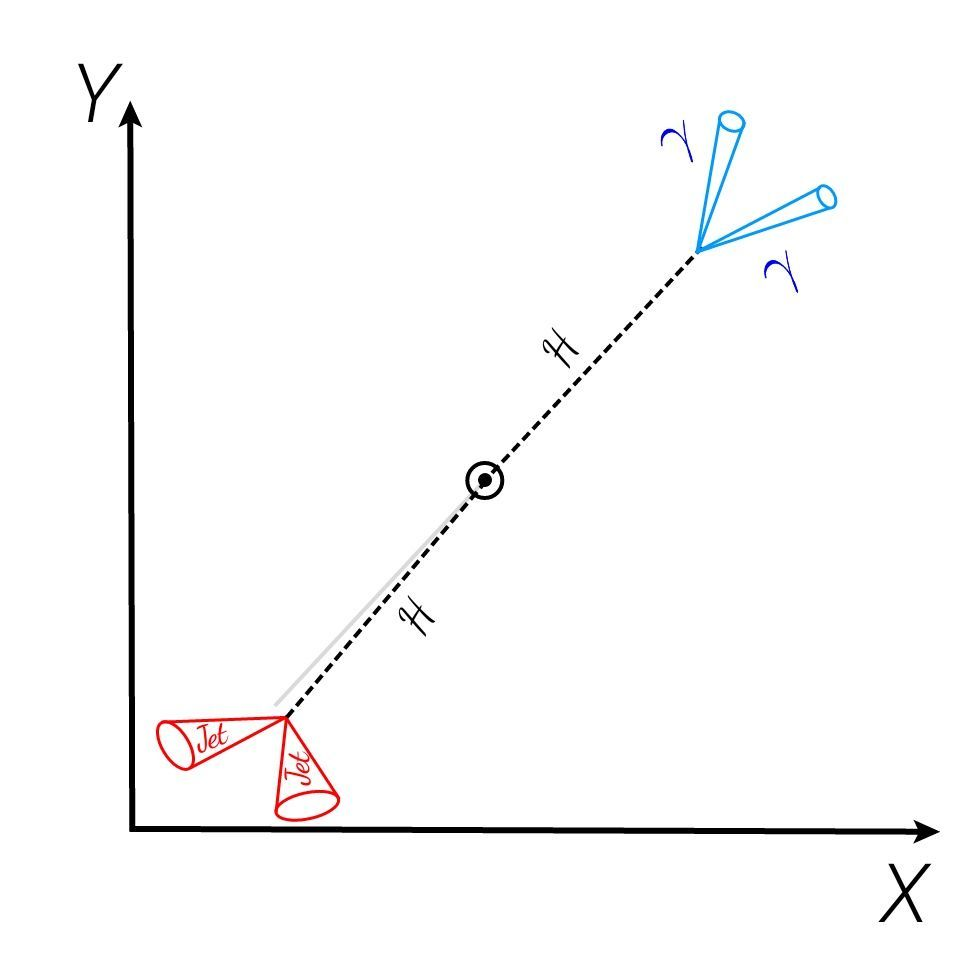
\includegraphics[width=.8\textwidth]{BackUp/Part7/Img/HH.png}
\end{figure}
    
\end{columns}  

\begin{equation*}
-2 \log (\mathcal{L})=\sum_{i}\left(\frac{\Omega_{i}^{*}-\Omega_{i}}{\sigma_{\Omega_{i}}}\right)^{2}-2 \log \left(L\left(p_{T}\right)\right)+\left(\frac{\sum p_{x}^{*}-0}{\sigma_{\sigma_{b b} \gamma \gamma}}\right)^{2}+\left(\frac{\sum p_{y}^{*}-0}{\sigma_{\sigma_{b \bar{b} \gamma \gamma}}}\right)^{2}
\end{equation*}    
\end{frame}

\begin{frame}{$\sigma_{b \bar{b} \gamma \gamma}$ determination}
\begin{columns}
\column{0.5\textwidth}
\begin{figure}
    \centering
    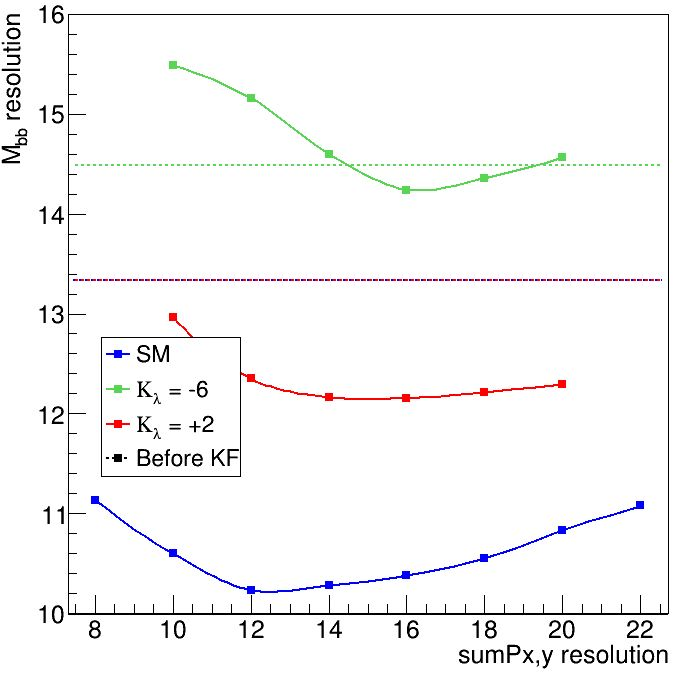
\includegraphics[width=1.\textwidth]{BackUp/Part7/Img/0JetScan.png}
\end{figure}
\column{0.5\textwidth}
\begin{figure}
    \centering
    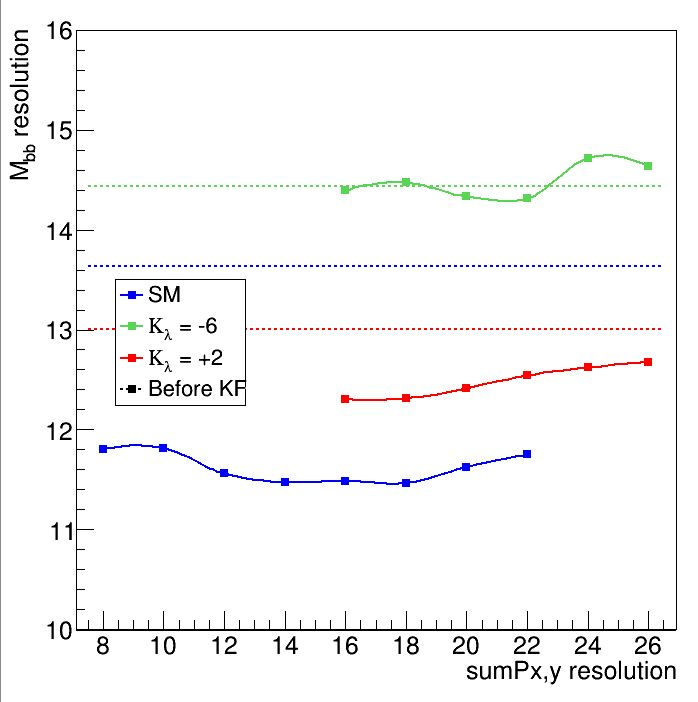
\includegraphics[width=1.\textwidth]{BackUp/Part7/Img/1JetScan.png}
\end{figure}
\end{columns}
\end{frame}

\begin{frame}{HH system balance}

\begin{columns}
\column{0.5\textwidth}
\begin{figure}
    \centering
    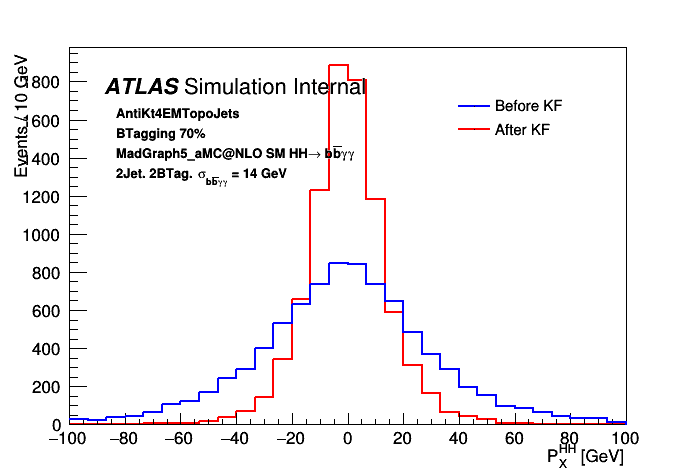
\includegraphics[width=1.\textwidth]{BackUp/Part7/Img/pxhh_KF_2Jet_AntiKt4EMTopoJets.png}
\end{figure}
\column{0.5\textwidth}
\begin{figure}
    \centering
    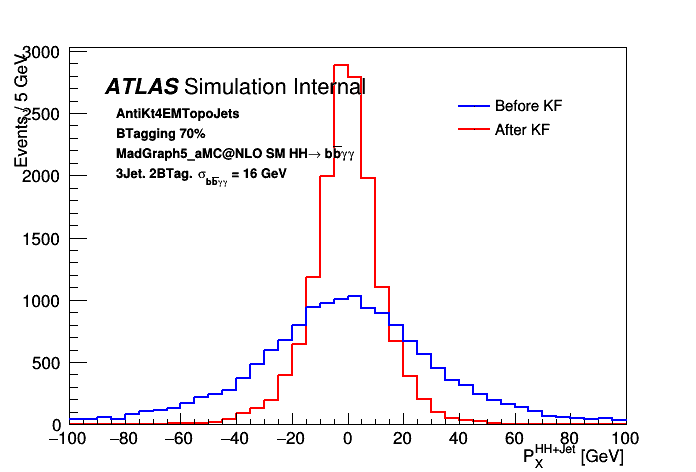
\includegraphics[width=1.\textwidth]{BackUp/Part7/Img/pxhh_KF_3Jet_AntiKt4EMTopoJets.png}
\end{figure}
\end{columns}
\end{frame}

\begin{frame}{$m_{bb}$ improvement}

\begin{columns}
\column{0.5\textwidth}
\begin{figure}
    \centering
    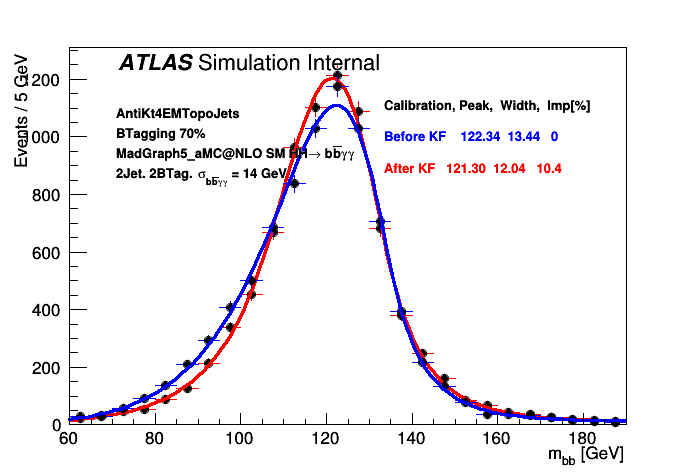
\includegraphics[width=1.\textwidth]{BackUp/Part7/Img/mbb_KF_2Jet_AntiKt4EMTopoJets.png}
\end{figure}
\column{0.5\textwidth}
\begin{figure}
    \centering
    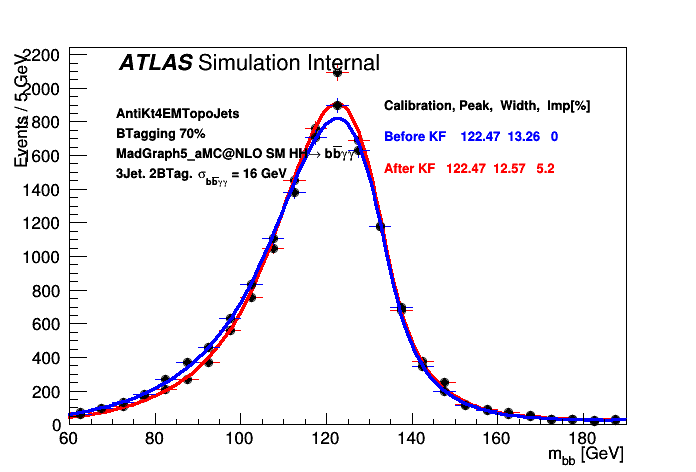
\includegraphics[width=1.\textwidth]{BackUp/Part7/Img/mbb_KF_3Jet_AntiKt4EMTopoJets.png}
\end{figure}
\end{columns}
\end{frame}
\begin{frame}{}
    
\end{frame}